\documentclass{standalone}

\usepackage{circuitikz}

\begin{document}

% INT_AY22_L24_Fig01_Rel_pos_vec.png

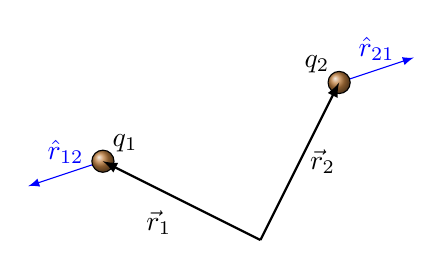
\begin{tikzpicture}[> = latex]

	% Unit vectors
	
	\draw [->, blue] (-2, 1) -- node [midway, above] {${\hat r}_{12}$} ++ ({180 + atan(1/3)} : 1);
	\draw [->, blue] (1, 2) -- node [midway, above] {${\hat r}_{21}$} ++ ({atan(1/3)} : 1);

	% Two masses
	
	\draw [ball color = brown] (-2, 1) circle (4 pt) node [above right] {$q_1$};
	\draw [ball color = brown] (1, 2) circle (4 pt) node [above left] {$q_2$};
	
	% Position vectors

	\draw [->, thick] (0, 0) -- node [midway, below left] {${\vec r}_1$} (-2, 1);
	\draw [->, thick] (0, 0) -- node [midway, right] {${\vec r}_2$} (1, 2);

\end{tikzpicture}

\end{document}